\documentclass[../main.tex]{subfiles}
\begin{document}

\subsection{Global-best guided Quantum-inspired Tabu Search Algorithm with Not-gate (GNQTS)}
\textbf{What is GNQTS and its evolution}

\textbf{Flow chart of GNQTS}

\begin{figure}
    \centering
    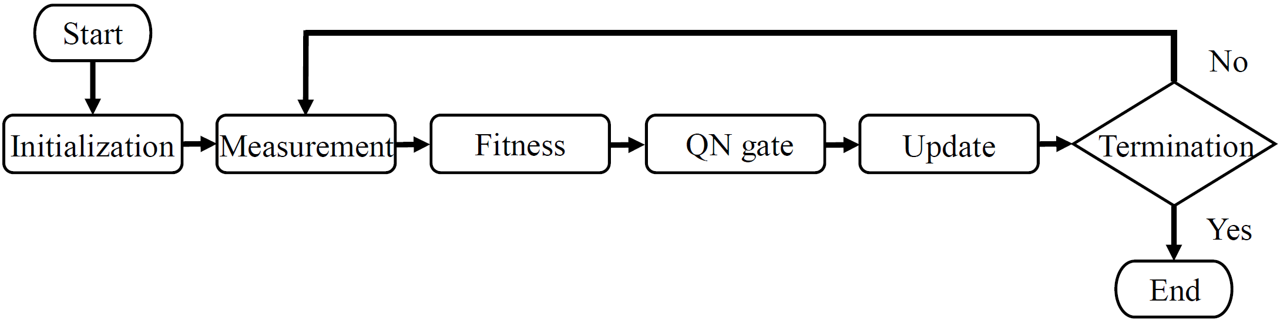
\includegraphics[scale = 0.5] {figure/flowChart.png}
    \captionsetup{font={footnotesize}}
    % \vspace{-3em}
    \caption{The flowchart of GNQTS}
    % \vspace{-0.5em}
    \label{flow}
\end{figure}

\textbf{Pseudo code of GNQTS}

\begin{algorithm}
    \caption{GNQTS}
    \begin{algorithmic}[1]
        \State $i \leftarrow 0$
        \State Initialize quantum  population $Q(0)$
        \State Initialize best solution $b$
        \While {not termination-condition}
        \State {$i \leftarrow i + 1$}
        \State Produce neighborhood set N by measure $Q(i-1)$
        \State Evaluate $f(s)$
        \State Find the best solution $s^b$ and the worst solution $s^w$
        \State Update $b$
        \State Detect whether GNQTS is stuck in local optimal
        \If {stuck}
        \State Do Quantum Not Gate
        \EndIf
        \State Update $Q(i)$
        \EndWhile
    \end{algorithmic}
\end{algorithm}
\bigbreak
\textbf{Explain each step of GNQTS}

\subsection{Sliding Windows}
\textbf{What are sliding windows}

\textbf{Old sliding sindows}

\textbf{New sliding windows}

\textbf{What can new sliding windows achieve}

\subsection{Technical Indicators}
% \textbf{What are technical indicators}

Technical indicators are the rule of thumb or pattern-based signals produced mathematically by the stock price or volume. The fundatioin of technical indicators is the historical prices of the stocks. It is belived that the history will repeated itself as the time extends. In other words, patterns of the market behavior continously appears throughout the history of the stock market. By analyzing the historical data, technical analysis use indicators to determine the timing to buy or sell stocks.

\subsubsection{Moving Average (MA)}

% \textbf{What is Moving Average}
A Moving Average is an indicator that shows the trend of stock price of a company. If the moving average was decreasing, it indicates that the price is falling recently. If the moving average was increasing, it indicates that the price is rising recently. There are several different types of moving averages. The most popular one is the Simple Moving Average (SMA), which is the indicator that is used in this research. The main difference between the moving averages is that the weighting applies to the price of stocks when calculating the indicator.
\bigbreak

% \textbf{How to use MA}
The most common way to use MA is to compare the relationship between two MA trends, known as crossover. The way to define a crossover is that when plotting two different MA values, the first MA line crosses through the second MA line from the bottom. This is also referred to as a golden cross. On the other hand, a death cross is that when the first MA line crosses through the second MA line of from above. We can simplify the trading strategy of using these two MA into MA($MA_{1},\ MA_{2}$). Table \ref{trad_MA} shows the parameters of traditional MA that are frequently been use by investers. The combination of the traditional strategy is restricted. Only two types of strategies are allowed, MA(Short-term, Mid-term), MA(Mid-term, Long-term). Hence there are 8 strategies in traditional MA.
\bigbreak

\begin{table}
    \centering
    \captionsetup{font={footnotesize}}
    \caption{Tradition MA strategies}
    \label{trad_MA}
    \footnotesize
    \begin{tabular*}{0.8\textwidth}{c @{\extracolsep{\fill}} cc}
        \toprule
        \textbf{Short-term}  & \textbf{Mid-term}      & \textbf{Long-term}   \\
        \midrule
        5 days (one week)   & 20 days (one month)    & 120 days (half year) \\
        10 days (two weeks) & 60 days (three months) & 240 days (one year)  \\
        \bottomrule
    \end{tabular*}
\end{table}

% \begin{table}
%     \centering
%     \captionsetup{font={footnotesize}}
%     \caption{Tradition MA strategies}
%     \label{trad_MA}
%     \footnotesize
%     \resizebox{0.5\textwidth}{!}{%
%         \begin{tabular}{ccc}
%             \toprule
%             \textbf{Short-term}  & \textbf{Mid-term}      & \textbf{Long-term}   \\
%             \midrule
%             5 days (one week)   & 20 days (one month)    & 120 days (half year) \\
%             10 days (two weeks) & 60 days (three months) & 240 days (one year)  \\
%             \bottomrule
%         \end{tabular}%
%     }
% \end{table}

% \begin{table}
%     \centering
%     \captionsetup{font={footnotesize}}
%     \caption{Tradition MA strategies}
%     \label{trad_MA}
%     \footnotesize
%     \begin{tabularx}\linewidth{ccc}
%         \toprule
%         \textbf{Short-term}  & \textbf{Mid-term}      & \textbf{Long-term}   \\
%         \midrule
%         5 days (one week)   & 20 days (one month)    & 120 days (half year) \\
%         10 days (two weeks) & 60 days (three months) & 240 days (one year)  \\
%         \bottomrule
%     \end{tabularx}%
% \end{table}
\bigbreak

% \textbf{SMA formula}
Amoung all the MA, SMA is a indicator which can be easily calculated, since the weight which applies to the price of stocks when calculating SMA is equally weighted. SMA is the average closed price of a certain period of time (e.g., 5 days). The period of days that is been used to calculate the averge price is called look-back period. The formula of SMA is shown in \ref{SMA}, where $N$ is the look-back period and $T$ is the date of today.

\begin{equation}\label{SMA}\scalebox{1}
    {$SMA_{N} = \dfrac{price_{T-N}+price_{T-N+1}+price_{T-N+2}+...+price_{T-2}+price_{T-1}}{N}$}
\end{equation}
\bigbreak

\bigbreak
Figure \ref{cross_demo} demostrate the timimg of golden cross and death cross when using SMA(5, 20). A buy signal is triggered when a golden cross appears. A selling signal is triggered when a death cross appears. These two types of crossover are the important signal to determine the timing of buying or selling the stocks.
\bigbreak


\begin{figure}
    \centering
    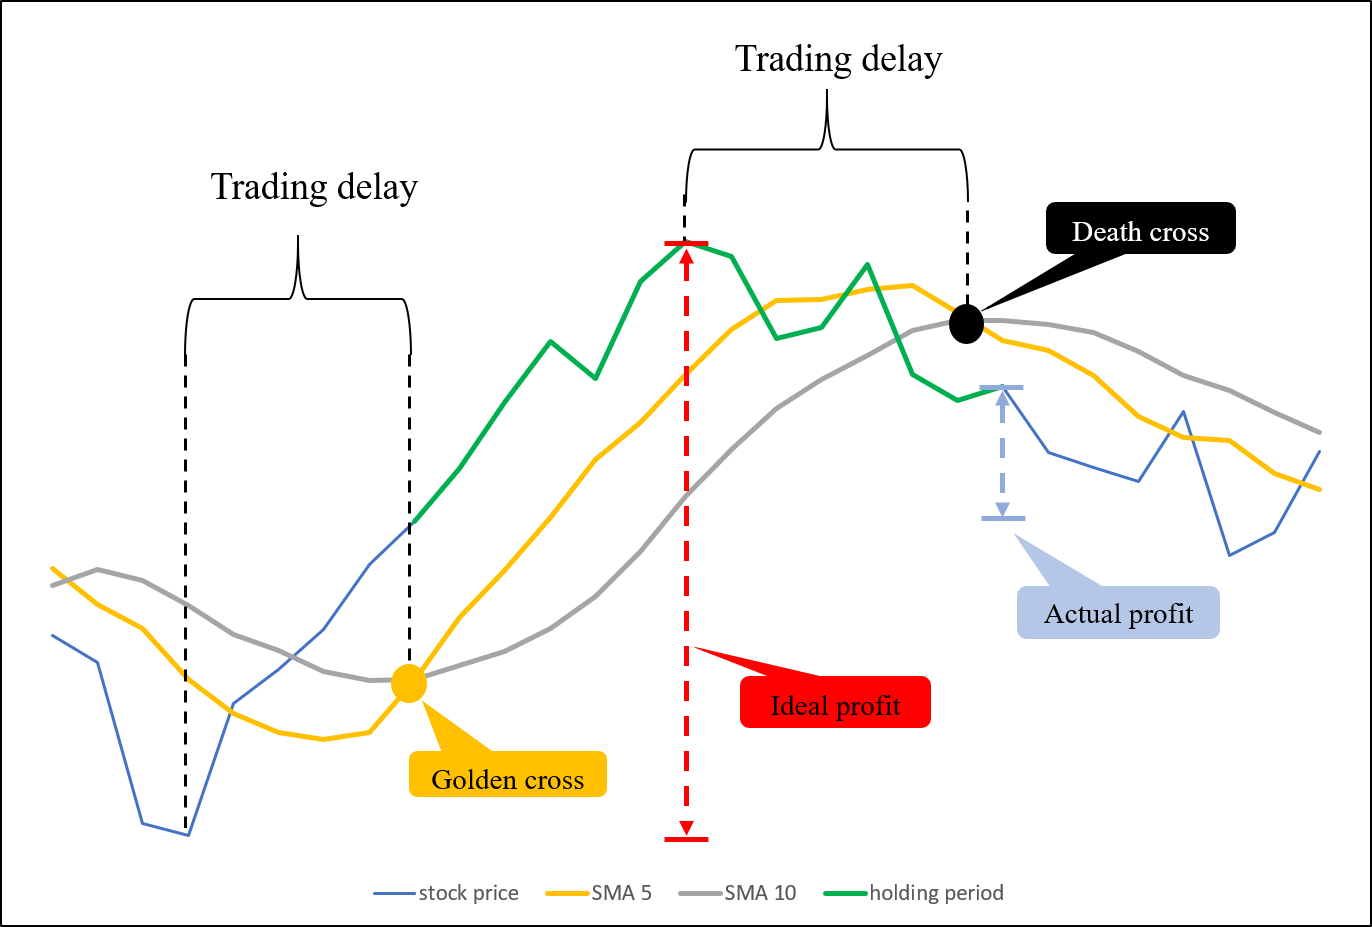
\includegraphics[scale = 0.6] {figure/cross1.png}
    \captionsetup{font={footnotesize}}
    % \vspace{-3em}
    \caption{Demostration of using strategy SMA(5, 20)}
    % \vspace{-0.5em}
    \label{cross_demo}
\end{figure}

% \textbf{Characteristics of MA}inconsistentparameters
Even though MA is a popular investment indicator, there are still some downsides. The first issue is that moving average is a lagging indicator. As we can see in figure \ref{cross_demo}, the golden cross and death cross are lagging behind the best time to buy or sell shares, leading to lower profits. The second issue is that there are too few traditional strategies. It is difficult to make a profit with just those few strategies. The third problem has to do with the lack of parameters. MA uses just two parameters to find the golden cross and the death cross. Using the same parameters to buy and sell does not appear to be sufficient.
\bigbreak
In order to break the boundaries of traditional MA strategy and find more accuate buying and selling point, this study extands the parameters of MA. There will be four parameters, two for buying and two for selling, rather than jus two for buying and selling. In addition, the parameters can be selected from 1 to 256, instead of choosing from short-term, mid-term and long-term.
This significantly increases the number of strategies from 8 to $\text{256}^\text{4}$. More than 4.2 billion strategies that can be selecte when using MA as indicator. Comparison of Traditoinal strategy and new MA strategy are shown in table \ref{trad_and_GN}.
\bigbreak

\begin{table}
    \centering
    \captionsetup{font={footnotesize}}
    \caption{Comparison of Traditoinal strategy and new MA strategy}
    \label{trad_and_GN}
    \footnotesize
    \begin{tabular*}{0.8\textwidth}{c @{\extracolsep{\fill}} cc}
        \toprule
        \textbf{}&\textbf{Traditoinal strategy}  & \textbf{new MA strategy}\\
        \midrule
        strategy  & MA($MA_1,\ MA_2$) & MA($MA_{buy_{1}},\ MA_{buy_{2}},\ MA_{sell_{1}}, \ MA_{sell_{2}}$) \\
        solution space& 8 & $\text{256}^\text{4}$  \\
        \bottomrule
    \end{tabular*}
\end{table}

\subsubsection{Relative Strength Index (RSI)}
\textbf{What is RSI}

Relative Strength Index (RSI) is a momentum oscillator that was first introduced by J. Welles Wilder, Jr. [3] in 1978. This is a popular indicator in financial technical analysis for calculating the recent price changes. RSI regards a rising stock price as strength from buyers, a falling price as strength from sellers, and the closing price is the outcome of the relative strength of buyers and sellers.
\bigbreak
\textbf{How to use RSI}

\textbf{Characteristics of RSI}

\textbf{RSI formula}

Here are the formulae for calculating RSI. The calculating process can be divided into two steps. For step one (as shown in formulae \ref{step_1}), the average gain and loss is the average of rice and drop respectively during the look-back period. As for step two, with the RSI in step one, we can recursively calculate the next RSI using formula 2, where $N$ is a parameter, representing a look-back period. The formulas for calculating RSI are as follows.

\begin{equation}\label{step_1}\scalebox{1}
    {$RSI_{step\ one}=100-\left[\dfrac{100}{1+\dfrac{Average\ gain}{Average\ loss}}\right]$}
    \vspace{1em}
\end{equation}

\begin{equation}\label{step_2}\scalebox{1}
    {$RSI_{step\ two}=100-\left[\dfrac{100}{1+\dfrac{Previous\ Average\ Gain\times(N-1)+Current\ Gain}{-(Previous\ Average\ Loss)\times(N-1)+Current\ Loss}}\right]$}
    \vspace{1em}
\end{equation}

\subsection{Normalize Internal Rate of Return}
How to evaluate the performance of our method

% \subsection{Investment Targets}
% what are DJI 30s

% what is DJI

% what is IXIC

% what is NYA

% Why choose these investment targets


\end{document}